%!TEX encoding = UTF-8 Unicode
% !TeX spellcheck = en_GB

%%%%%%%%%%%%%%%%%%%%%%%%%%%%%%%%%%%%%%
\chapter{ Overview of Higgs pair production at colliders }\label{chap:overviewDiHiggs}
%%%%%%%%%%%%%%%%%%%%%%%%%%%%%%%%%%%%%%
The determination of the shape of the Higgs potential is an essential part of the LHC physics programme. Unlike other Higgs measurements reviewed in this thesis, the light Yukawa and Higgs-self couplings  are exceptionally hard to probe.  This is particularly evident from the conclusion of ~\autoref{chap:4topSingleHiggs}. When we have seen that the effectiveness of using single-Higgs signals in order to probe the Higgs trilinear coupling is challenged by other weakly constrained operators also effecting these signals. Thus, Higgs pair production remains as the only direct way to access this elusive interaction. \\ The production of Higgs in pairs has roughly~$ 10^{-4} $ the signal of producing a single Higgs at the LHC. Higgs pair production, with Higgs decays considered, has a cross-section of $ \sim 1 \si{\femtobarn}$, in the SM. This makes it inaccessible from Run-II or Run-III data, but should be accessed using the whole luminosity of the HL-LHC ~\cite{Apollinari:2015bam,ATL-PHYS-PUB-2018-053,Cepeda:2019klc}. As for the quartic coupling, that requires NLO corrections to Higgs pair or triple Higgs production, both of which are beyond the sensitivity of the LHC~\cite{Plehn:2005nk}. The measurement potentials for the light Yukawa couplings shall be discussed in the Next chapter.   The main advantages for Higgs pair production in determining the Higgs trilinear self-coupling comes from the dependence of the cross-section on $\lambda_3$ at the LO level, as well as the fact that the rest of SMEFT operators entering in this process~(see eq~\eqref{HH-smeft}) can be strongly constrained from other processes, breaking any potential correlations that might appear between them and the trilinear coupling using only di-Higgs data. However, the inclusion of light quark Yukawa couplings modifiers e.g. $ C_{u\phi}$ and $C_{d \phi}$ would complicate things as we shall see in~\autoref{chap:lightyuk}. \\
This chapter will start by reviewing the theoretical status of the dominant process for Higgs pair production, starting with the gluon fusion in~\autoref{ggFhh}. Then, the other subdominant channels will be briefly reviewed in~\autoref{otherhh}. I will afterwards overview the experimental efforts in probing this rare yet fascinating processes in~\autoref{exphh}. Finally, I will present  in~\autoref{summtrilinear} a summary of the potential for Higgs production in probing Higgs elusive interactions.
%%%%%%%%%%%%%%%%%%%%%%%%%%%%%%%%%%
\section{Higgs pair production by gluon fusion \label{ggFhh}  }
%%%%%%%%%%%%%%%%%%%%%%%%%%%%%%%%%%
The dominant process for Higgs pair production at the LHC~(and hadron colliders in general) is the gluon fusion channel via top quarka in the loops, while the beauty quark loops contribute only to~$1\%$, as shown in~\autoref{fig_ggf_sm}.
%
\begin{figure}[!htpb]
	\centering
	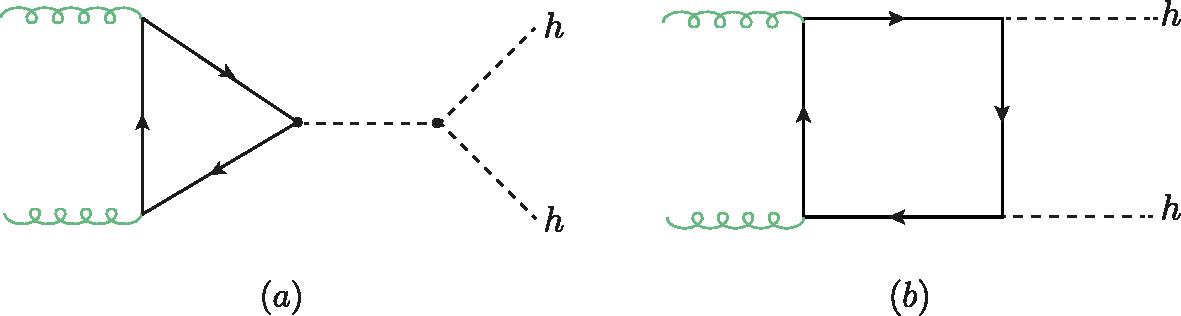
\includegraphics[width = 0.8\textwidth]{./figures/di-higgs-LO-SM}
	\caption{Feynman diagrams for the ggF process of Higgs pair production in the SM.} 
	\label{fig_ggf_sm}
\end{figure}
%
This process is well-studied at leading order~(LO) analytically~\cite{EBOLI1987269,GLOVER1988282,DICUS1988457,Plehn:1996wb}.  The higher order computations are significantly more complicated to preform compared to the gluon fusion production of single-Higgs. This is due to the fact that multi-scale amplitudes at two-loops (and more) cannot be always computed analytically using the current computational techniques.  The first attempt to compute the NLO corrections to di-Higgs were via the HTL approximation~\cite{Dawson:1998py, Altenkamp:2012sx,Grigo:2014jma} and implemented in~\texttt{HPAIR}~\cite{Plehn:1996wb}. These corrections were found to be large, with a K-factor of $ \sim 2$.  This prompted more calculations with inclusion of top mass effects~\cite{deFlorian:2013uza,Grigo:2013rya,Maltoni:2014eza,Grigo:2015dia,Degrassi:2016vss}, which improved the stability of the HTL expansion as well as corrected the cross-section by $\sim 10\%$. In addition, the threshold resummation effects of the HTL have been included in \cite{Shao:2013bz}. This approach, however, is not sufficient to produce corrections to the differential cross-section, as the HTL fails for $m_{hh}^2/4m_t^2 \lesssim 1$. Using numerical evaluation of the two-loop integrals, it is possible to obtain exact results with full top mass dependence, see refs.~\cite{Borowka:2016ypz,Borowka:2016ehy,Baglio:2018lrj}. Nonetheless, this comes at the cost of computational power required to evaluate the cross-section.  Hence, approximation methods were essential to obtaining more flexible results for use at simulations and BSM Higgs pair production.  These approximations methods are analogous, and sometimes connected  to the ones used for $Zh$ production discussed in~\autoref{chap:hz}. This includes, small final particle transverse momentum~\cite{Bonciani:2018omm}, and high energy~(HE) expansions~\cite{Davies:2018ood}. In addition to a method developed in refs. ~\cite{Xu:2018eos,Wang:2020nnr} which considers both $\hat s , \hat t$ and $m_t$ as large quantities while keeping the Higgs mass as small one. This method has a wide coverage of the $m_{hh}$ spectrum.  The use of Pad\'e approximation to improve the $\pt$--expanded amplitude coverage as well as to obtain a description for the three-loop~(NNLO) form factors was demonstrated in~\cite{Davies:2019nhm}. The NNLO cross section with top mass effects has been computed numerically in~\cite{Grazzini:2018bsd} and also at differential level~\cite{deFlorian:2016uhr}, and analytically only in the HTL~\cite{deFlorian:2013jea}. Also, NLO+ NNL analytic results have been obtained by~\cite{deFlorian:2015moa}. Parton shower matching for NLO Higgs pair production has been computed  in~\cite{Jones:2017giv,Heinrich:2019bkc}, which was essential for the \texttt{POWHEG} implementation for di-Higgs, with NLO corrections computed from a grid has been made available by ~\cite{Heinrich:2017kxx,Heinrich:2019bkc,Heinrich:2020ckp}. \autoref{dihiggs-gridplot} shows the Higgs pair virtual partonic cross-section defined in~eq.\eqref{eq:deltasigma} vs the  $\pt$ and HE expansions bridged using Pad\'e  approximants~\cite{Bellafronte:2022jmo}.  The matching between the results across low and high energy intervals of $m_{hh}$ shows the strength of Pad\'e  approximants technique.  This is the most recent analytic higher order correction result for Higgs pair production.\\
%
The LO Higgs pair production with SMEFT operators is available in \texttt{SMEFTatNLO} model~\cite{Degrande:2020evl} for ~\texttt{MadGraph}.

\begin{figure}[!htpb]
	\centering
	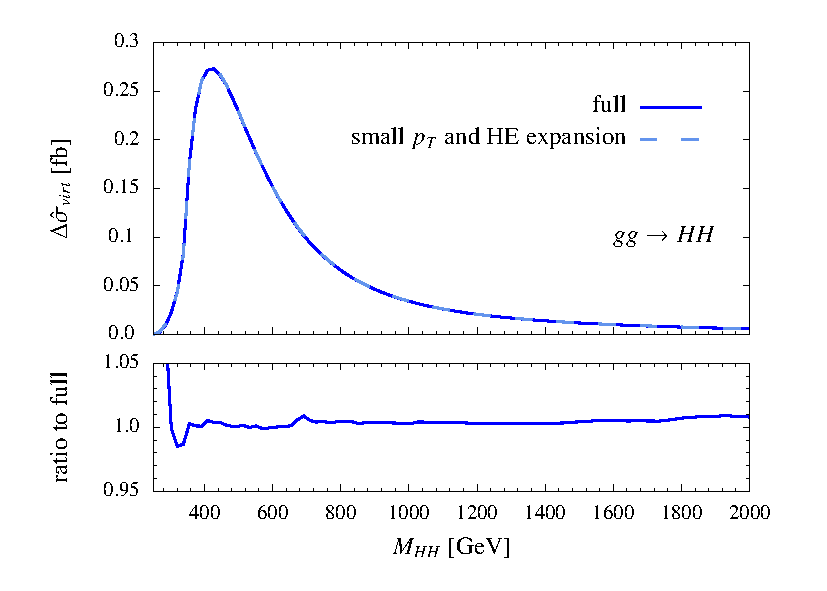
\includegraphics[width = 0.8\textwidth]{./figures/HH_NLO}
	\caption{Combination of the HE and $\pt$ expansions of the virtual two-loop NLO corrections using  Pad\'e  approximants,  confronted with the NLO results from a numerical grid. This plot is taken from~\cite{Bellafronte:2022jmo}. } 
	\label{dihiggs-gridplot}
\end{figure}
%
%%%%%%%%
Calculation of LO in addition to Higher order corrections to Higgs pair production in EFT, MSSM and composite Higgs models can be found in~\cite{Grober:2010yv,Grober:2014zva,Grober:2015cwa,Grober:2017gut,deFlorian:2017qfk,Buchalla:2018yce}.\\ 
The NNLO correction were used according to the Higgs cross section working group recommended values~\cite{Dittmaier:2012vm,deFlorian:2016spz}:
\begin{equation}
	K = \frac{\sigma_{NNLO}}{\sigma_{LO}}, \;\;\;\;\; K_{14 \mathrm{TeV}} \approx 1.71.
\end{equation}
\subsection{Theoretical uncertainties}
There are four main sources of theoretical uncertainties for Higgs pair production:
\begin{enumerate}
	\item Scale uncertainty: coming form the arbitrariness of scales choice.
	\item PDF uncertainties: coming form the uncertainty in the PDF fitting and model.
	\item $\alpha_s$ running uncertainty: originating from the initial value (i.e. $\alpha_s(M_Z) $).
	\item Top mass renormalisation scheme, which involves $m_t$ appearing in the loop propagators and in the top Yukawa.
\end{enumerate}
The computation of the uncertainties is described in ~\cite{Martin:2009bu, Demartin:2010er}. for PDF and $\alpha_s$ uncertainties.
In order to calculate the scale uncertainties, the cross-section was computed with different $ \mu_R$ and $\mu_F$ values ranging between:
\begin{equation}
	\frac{M_{hh}}{4} \leq \mu_R/\mu_F  \leq \,M_{hh}
\end{equation}
As for the $m_t$ renormalisation uncertainty, one uses the $\MSbar$ running of the top mass formula at N$^3$LO~\cite{Baglio:2020wgt}
\begin{equation}
	\overline{m_t} (m_t^{pole}) =m_t^{pole}\, \left( 1+\frac{4}{3 \pi} \alpha_s(m_t^{pole})+10.9 \frac{\alpha^2_s(m_t^{pole})}{\pi^2} +107.11 \frac{\alpha^3_s(m_t^{pole})}{\pi^3}. \right) ^{-3} 
\end{equation}
The total 14 TeV ggF $hh$, cross-section at different orders in computation with its uncertainties are shown in~\autoref{ggf_xsres}, which indicates that the uncertainties are dominated by the $m_t$ renormalisation scheme of $\sim -18\%$ uncertainty in the lower envelope.  This is significant part of the uncertainty budget and needs to be resolved by including N$^3$LO corrections to ggF $hh$, such corrections are available in the  HTL~\cite{Chen:2019lzz,Chen:2019fhs}. 
%
\begin{table}
	\centering
	\begin{tabular}{ccccc}
		\toprule
		& $ \sigma$	[fb] & Scale [fb] & PDF$+\alpha_s$ [fb]& Total [fb] \\
		\midrule
		SM HEFT  (LO)      &  $ 18.10$    &   $-$      & $-$   &  $-$ \\
		SM   running mass (LO)  &  $ 16.96$    &   $ -$   & $-$   &  $-$ \\
		SM    (LO)  &  $ 21.45$    &   $ \,^{+4.29}_{-3.43}$   & $\pm 1.46$   &  $ \,^{+4.53}_{-3.73}$ \\
		SM   (NLO)~\cite{Baglio:2012np}  &  $ 33.89$   &   $ \,^{+6.17}_{-4.98}$   & $ \,^{+2.37}_{-2.01}$   &  $ \,^{+6.61}_{-5.37}$ \\
		SM   (NNLO)~\cite{Grazzini:2018bsd}  &  $36.69$    &    $ \,^{+0.77}_{-1.83}$   & $\pm 1.10$   &  $ \,^{+1.66}_{-6.43}$ {\tiny(incl. $m_t$ uncertainty~\cite{Baglio:2020wgt})} \\
		\bottomrule
	\end{tabular}
	\caption{Gluon fusion~(ggF) Higgs pair production cross-section at 14 TeV with theoretical  uncertainties, the HTL is computed using HEFT, top running mass, LO, NLO and NNLO QCD corrections. The NLO and NNLO results are taken from the references cited in the table. The LO results are computed via a FORTRAN code.}
		\label{ggf_xsres}
\end{table}

\section{Other processes\label{otherhh}  }
Like  single-Higgs production at hadron colliders, the production of Higgs pairs has the same subdominant channels VBF, di-Higgsstrahlung $ Vhh$ and associates production of Higgs pair with tops $t\bar hh /t j hh$. Their cross-sections and uncertainties at 14 TeV are shown in~\autoref{table:di-higgs}, while in~\autoref{dihiggs-all} their cross-sections as a function of the centre-of-mass energy $\sqrt{s}$ is shown~\cite{DiMicco:2019ngk}. 
\begin{table}[htbp!]
	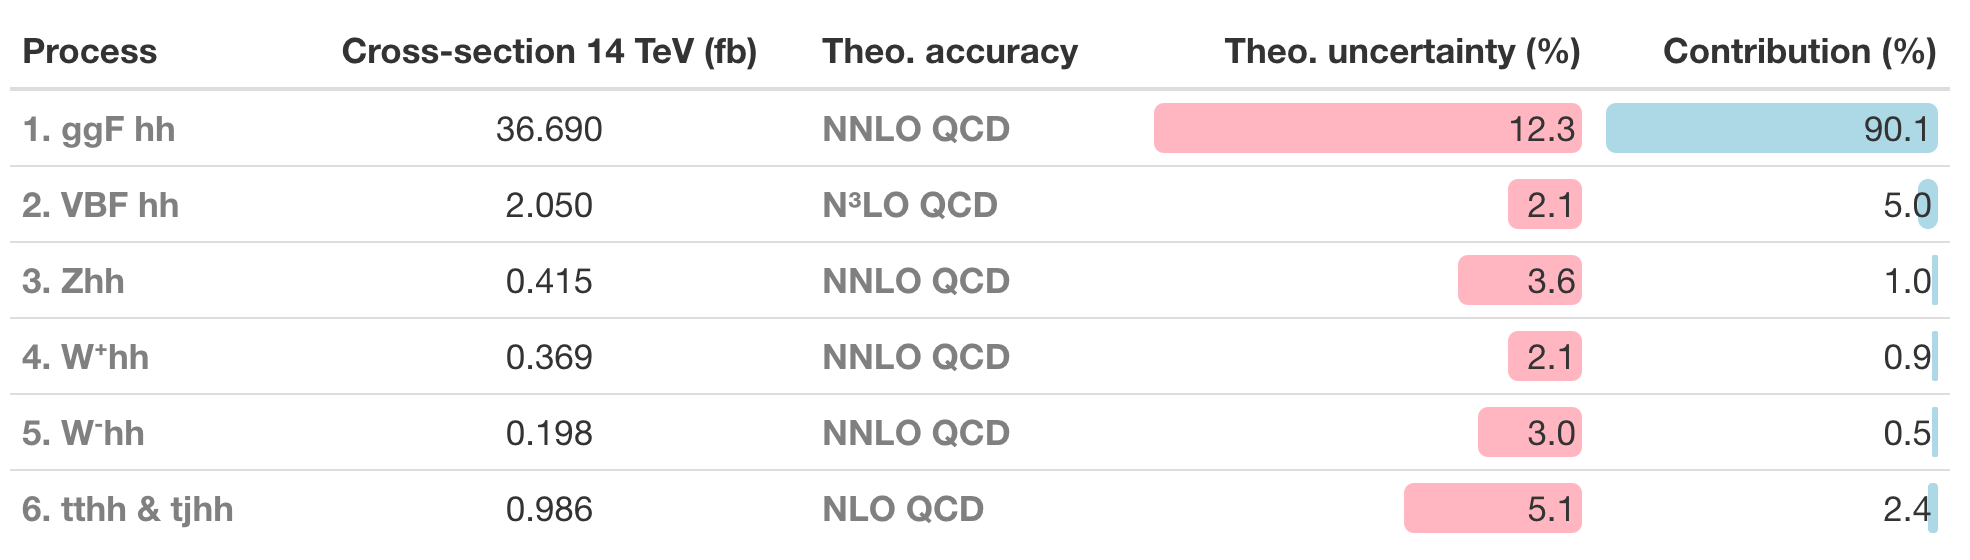
\includegraphics[width=1\textwidth]{hh-table}
	\caption{ Summeray of the Higgs pair production processes at 14 TeV LHC. \label{table:di-higgs} }
\end{table}
\subsection{VBF $hh$}
Vector boson fusion $hh$ production has the second largest cross-section after ggF $hh$, which is calculated up to N$^3$LO~\cite{Baglio:2012np,Ling:2014sne,Dreyer:2018qbw} inclusively and differentially at NNLO~\cite{Dreyer:2018rfu}. The dominant diagrams are analigious to the single Higgs VBF, which involve the $W/Z$ bosons exchanged in the $t-$channel. The process has the same topology as the -off shell- single Higgs VBF, with the off-shell Higgs giving two final states ones via the trilinear self-coupling. 
\subsection{Di-Higgsstrahlung}
The associated production of Higgs pair with $W$ and $Z$ bosons has a small cross-section compared to ggF and VBF,  this process is known up to NNLO QCD accuracy, which includes the gluon-fusion component in the full computation~\cite{Li:2016nrr,Li:2017lbf}. 
\subsection{Associated Higgs pair production with $t$-quarks}
Sometimes called the di-Higgs bremsstrahlung off top quarks~\cite{DiMicco:2019ngk}, this channel has a steeper dependence on $\sqrt{s}$ than the single Higgs bremsstrahlung $t\bar t h$. One can see, for example, from ~\autoref{dihiggs-all} that its cross-section becomes at  roughly the same  values as the VBF's. Only NLO computations for this channels have been carried out~\cite{Frederix:2014hta}. \\ All of the three channels have a relatively small NLO correction, compared to ggF, which ranges from 10-30\%. 
\begin{figure}[!htpb]
	\centering
	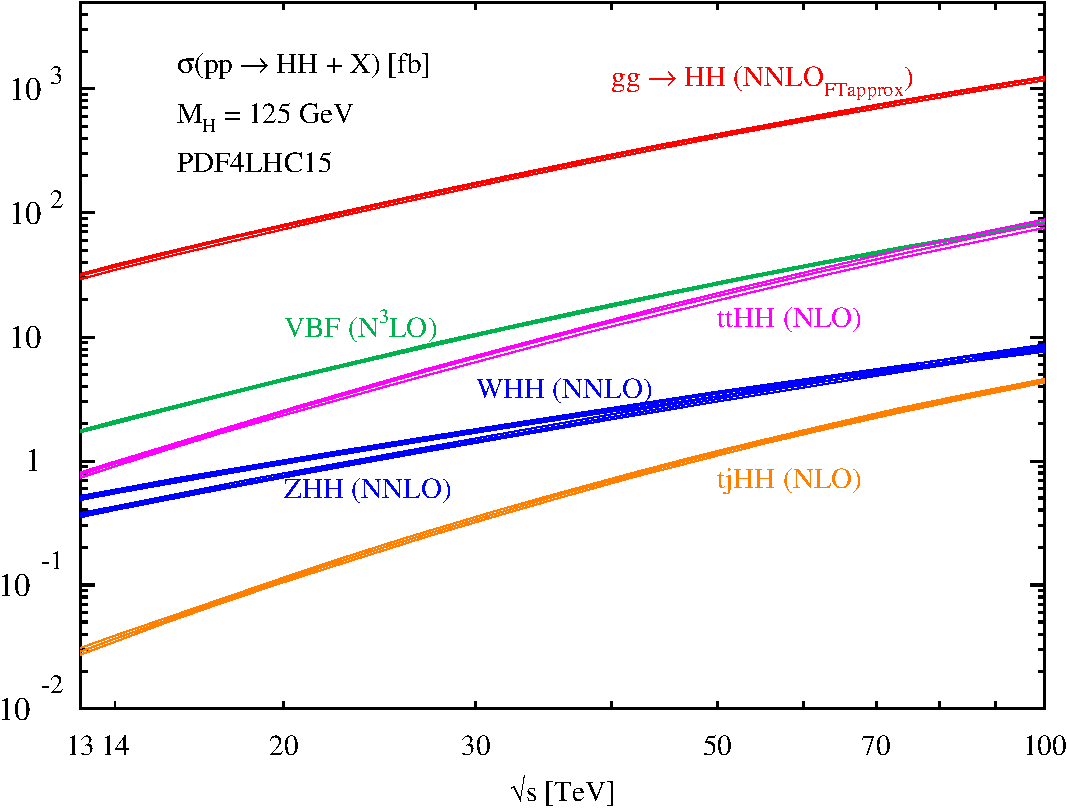
\includegraphics[width = 0.8\textwidth]{./figures/cxn_HH}
	\caption{The cross-section of all di-Higgs processes at the highest available perturbation order as a function of centre-of-mass energy $\sqrt{s}$.The bands show the uncertainties without the top-mass renormalisation scheme. This plot is taken from~\cite{DiMicco:2019ngk}.} 
	\label{dihiggs-all}
\end{figure}
%
%%%%%%%%

\section{Experimental overview for Higgs pair production \label{exphh}  }
The search for Higgs pair production can be divided into two categories, resonant and non-resonant searches. The first searches for heavy resonances that decay into a Higgs pair, while the latter is concerned about the SM or if NP scale beyond the reach of the LHC, i.e. when the EFT limit is valid. In this review, I shall focus on the non-resonant searches, as these are the ones relevant to focus of this thesis, for detailed overview of the resonant searches cf.~\cite{DiMicco:2019ngk}.\\
%
\autoref{dihigs-exp} shows the current experimental scopes for detecting non-resonant Higgs pair production by both ATLAS and CMS. The searches are summarised according to the final state:
\begin{figure}[!htpb]
	\centering
	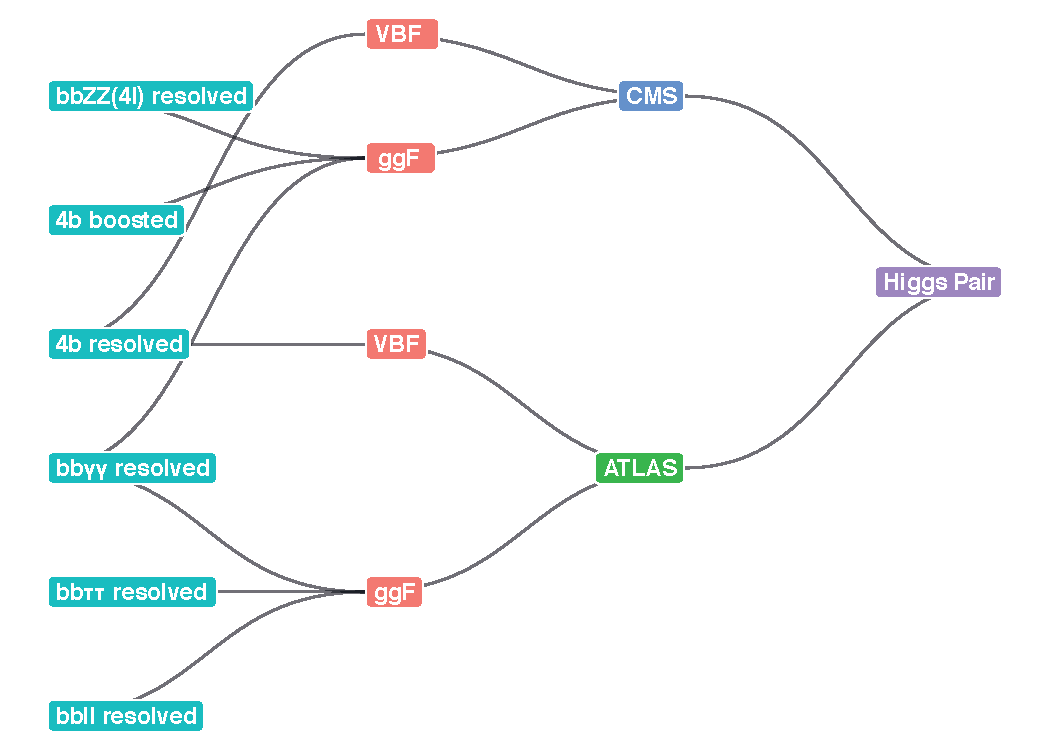
\includegraphics[width = 0.8\textwidth]{./figures/HH-exp-network}
	\caption{The non-resonant Higgs pair searches conducted by ATLAS and CMS using the full Run-II data.} 
	\label{dihigs-exp}
\end{figure}
\subsection*{$hh \to b\bar b b \bar b $}
 The final state $ hh \to b\bar b b \bar b$ has the highest SM cross-section possible for Higgs pair, but poses a difficulty due to the large QCD background  coming from the search for four b-tagged jets in the final state. CMS~\cite{CMS-PAS-HIG-20-005} has used Boosted decision trees~(BDT) for studying this final state for ggF and VBF channels, separated. This allowed for sensitivity on the trilinear and $hhVV$ coupling. This analysis led to 95\% CL bounds on $\kappa_\lambda \in [-2.3;9.4]$ and $\kappa_{2V} \in [-0.1; 2.2]$.  They have also preformed boosted analysis for the VBF channel, by defining two large jets with jet radius of $\Delta R =0.8$. Despite their analysis not being sensitive to the trilinear self-coupling, it could probe both $\kappa_V$ and  $\kappa_{2V} $, which leads to the most stringent bound on the latter coupling modifier so far  $\kappa_{2V}  \in [0.6;1.4]$. The $\kappa_{2V}=0$ hypothesis is excluded with $ p<0.001$~\cite{CMS-PAS-B2G-21-001}. On the other hand, ATLAS has preformed only a resolved analysis for this final state and for the VBF production channel~\cite{ATLAS:2020jgy}, hence they were able to report bounds on $hhVV$ coupling $\kappa_{2V} \in [-0.43;2.56]$. 
\subsection*{$hh \to b\bar b VV $}
ATLAS has considered the gluon fusion final state~$hh \to b\bar b \ell \ell$, with the leptons coming from $WW/ZZ$ decays~\cite{ATLAS:2019vwv}. This states covers around $90\%$ of the total~$hh \to b\bar b VV $ signal. Their analysis was divided into two categorise, same-flavour and different-flavour leptons. The observed signal strength were higher than the expected one. Hence, no bounds on the self-coupling could be extracted from this search. Similar analysis has been carried out by CMS, but with a requirement to observe four leptons instead of two, hence they searched for the final state $hh \to b\bar b( ZZ^*\to 4\ell)$. The 95\% CL upper limit on the signal strength was 30 times the SM one, with bounds on Higgs self-coupling of $\kappa_\lambda \in [-9;14]$~\cite{CMS-PAS-HIG-20-004}. 
\subsection*{$hh \to b\bar b \tau \tau $}
This channel has backgrounds coming from real $\tau$'s, such as $t\bar t$ and $Z j$ with heavy jets. In addition to fake $\tau$'s coming from QCD multijet process. A neural network~(NN) has been used by ATLAS~\cite{ATLAS-CONF-2021-052}investigating this channel, using resolved b jets. The extracted bounds on the trilinear self-coupling are $\kappa_\lambda \in [-2.4;9.2]$. 
\subsection*{$hh \to b\bar b \gamma \gamma $}
This final state is the most promising for Higgs pair searches. Despite having a lower cross-section that the previous final states with BR of  0.27\% in the SM, it has the highest selection efficiency.  This is due to the low backgrounds and the ability to fully reconstruct the photons. The dominant non-reducible background is QCD/QED production of $b\bar b \gamma \gamma$, which has a cross-section of ~$\sim13\si{\femtobarn}$ at the 14 TeV LHC, more details about the backgrounds of this final states are shown in~\autoref{tab:xsec14}. \\
\begin{table}[h!]
	\centering
	\begin{tabular}{cccc}
		\specialrule{.8pt}{0pt}{0pt}
		Channel	        &LO $\sigma$ [fb]	&NLO $K$-fact	&6$\inab$ [\#evt @ NLO]   \\ %& 2$b$-jets[\%]  \\ 
		\specialrule{.8pt}{0pt}{0pt}
		$b\bar b h, y_b^2$	        &0.0648	            &1.5	    &583                \\%&7.7\%  \\
		$b\bar b h, y_by_t$        &-0.00829	        &1.9        &-95                \\%&4.0\%	\\
		$b\bar b h, y_t^2$	        &0.123	            &2.5	    &1,840              \\%&12\%	\\
		$Zh$	        &0.0827	            &1.3	    &645                \\%&21\%   \\
		$\sum\bbh$	    &0.262	            &-	        &2,970              \\%&-      \\
		$\bbaa$	        &12.9	            &1.5	    &116,000            \\%&14\%	\\
		$t\bar th$	    &1.156	            &1.2	    &6,938              \\%&42\%	\\
		%$hh_{\rm SM}$	&0.567	\la{0.053}            &1.72	    &3,492  \la{316}              \\%&32\%	\\ 
		\specialrule{.8pt}{0pt}{2pt}
	\end{tabular}
	\caption{ SM cross-section for the main background processes at 14\ TeV with 6$\iab$ data at the HL-LHC. For $\bbh$ production, the Higgs boson is decayed to a pair of photons. The total production of Higgs associated with $b\bar{b}$ is denoted by $\sum\bbh$ and is the sum of the top four channels.
	}
	\label{tab:xsec14}
\end{table}
Both ATLAS and CMS have published searches of this channel using  BDT and NN analyses~\cite{ATLAS:2021jki,CMS:2020tkr}. With ATLAS reporting the strongest 95\% CL bound on $\kappa_\lambda$ thus far, which was used in the comparisons in~\autoref{fig:summcphihl-lhc}. While CMS has reported bounds on both $\kappa_\lambda$ and $\kappa_{2V}$ : $\kappa_{\lambda} \in [-3.3;8.5]$ and $\kappa_{2V} \in [-1.3; 3.5]$.                                                                                       
\subsection{Prospects for the HL-LHC}
The highlight of the HL-LHC programme is the detection of Higgs pair production. It is projected that the Higgs pair signal to be observed at $\sim  4- 4.5\sigma $ level~\cite{DiMicco:2019ngk}. The use of machine learning techniques in the analysis of $hh$ searches will be a key factor to the success of these searches~\cite{Cepeda:2019klc}. In~\autoref{sec:mlanalysisly} the interpretable machine learning technology will be exploited in improving the sensitivity for $hh$ signals at the HL-LHC. With the main focus on the $\bbaa$ final state. As this channel has the highest potential for discovery of di-Higgs production~\cite{Azatov:2015oxa, Baur:2003gp, Baglio:2012np, Kling:2016lay, Barger:2013jfa, Adhikary:2017jtu,Alves:2017ued}. The projected constraints on $\kappa_\lambda$ at the HL-LHC for combined ATLAS and CMS are~$\kappa_{\lambda} \in [0.1,2.3]$~\cite{DiMicco:2019ngk,Cepeda:2019klc}
 
\section{Summary \label{summtrilinear}  }
The Higgs pair production is a missing key measurement of the SM, it is essential for the determination of the Higgs potential by directly constraining the Higgs trilinear self-coupling. Moreover, this channel is sensitive to non-linear couplings of the Higgs, like $hhVV$ and $hh f\bar f$. Due to the small cross-section of this channel, current searches obtain rather weak bounds on $\kappa_{\lambda}$ that are comparable with the perturbative unitarity bounds~\cite{DiLuzio:2017tfn}. Nonetheless, the HL-LHC is expected to result in an observation or even discovery of this process, particularly with the help of advanced machine learning techniques.\\ The observation of Higgs pair production is expected to provide a direct measurement on one of the two ``difficult'' couplings in the SM Higgs sector,  the trilinear Higgs self-coupling. However, as we shall explore in the upcoming chapter, it could also provide a window for observing the Higgs coupling to light quarks, which is the second difficult coupling class we have talked about earlier.
